%%% Research Diary - Entry
\documentclass[11pt,a4paper]{article}

% Working date: The date this entry is describing. Not necessary the date of last edit.
\newcommand{\workingDate}{\textsc{@year $|$ @MONTH $|$ @dday}}

% Name and institution must preceed call to researchdiary.sty package
\newcommand{\userName}{Pierre Bréchet}
\newcommand{\institution}{TUM}

% The guts and glory
\usepackage{research_diary}
\usepackage{usrcmd}
\bibliography{bibliography}

% Begin document.
% Use \logoPNG or \logoEPS. If compiling with PDFTeX, use \logoPNG
\begin{document}
% \logoPNG

{\Huge @MONTH @day}

\section*{Gaussian}

The thesis results were not using batchnormalization in their layers. Tests that were made again were using batchnormlization.

ALI is using batch normalization in the generator, and not in the discriminators. This could be argued by the need of the generator to produce samples from an already normalize input, whereas the discriminator input is real data samples; using batch normalization in the discriminator would lead to a prolonged learning time (discriminant features would take longer to be learned ?)

Also, the $\beta_1$ parameter of the Adam optimizer in ALI is choosen randomly $\beta_1 = 0.8$, and $\beta_2$ is default $\beta_2 = 0.999$
The structure is similar to BidirectionalGAN (BiGAN) found in \cite{Donahue2016}.

\subsection{With no informative regularization}

When no regularization is used on the informative part, the learned
distribution suffers from blurry edges (even when using Sinkhorn). Using
antifinformative regularization corresponds to much sharper result.

\begin{figure}[!htbp]
   \centering
\begin{subfigure}[t]{0.48\textwidth}
   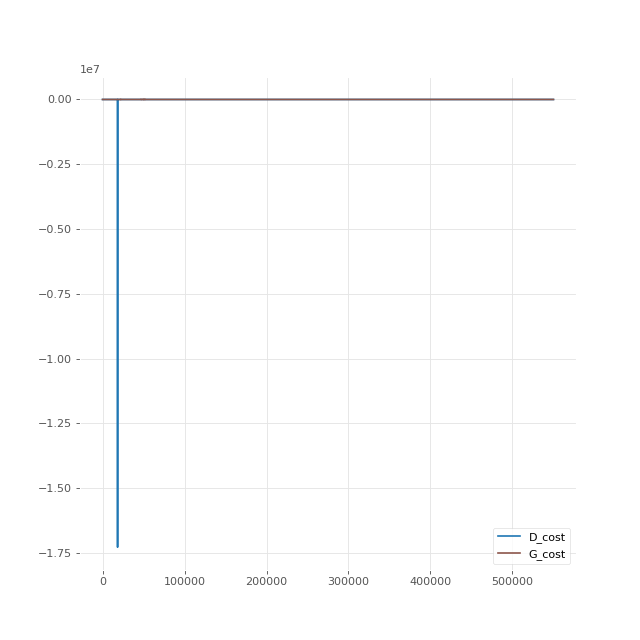
\includegraphics[width=\textwidth,center]{2019-04-30/mnist/info/plots/D_cost_G_cost.png}
   \caption{D_cost_G_cost.}
   \label{fig:.._.._notes_journal_figures_2019-04-30_mnist_info_plots-a}
\end{subfigure}
\begin{subfigure}[t]{0.48\textwidth}
   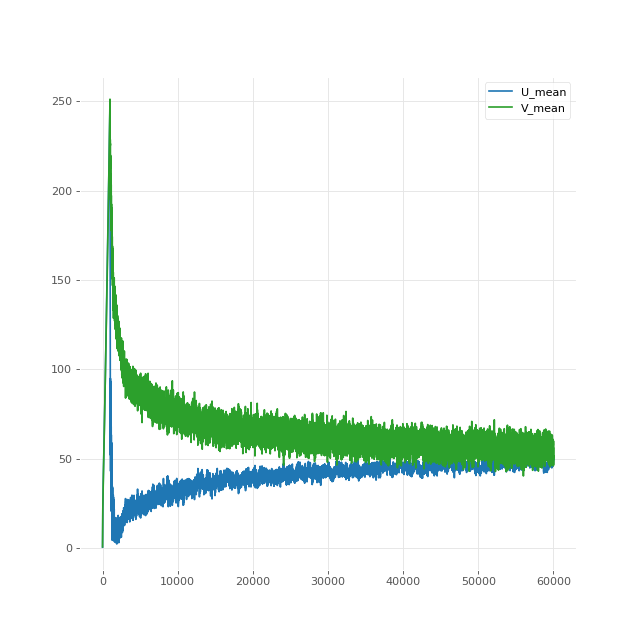
\includegraphics[width=\textwidth,center]{2019-04-30/mnist/info/plots/U_mean_V_mean.png}
   \caption{U_mean_V_mean.}
   \label{fig:.._.._notes_journal_figures_2019-04-30_mnist_info_plots-b}
\end{subfigure}
   \caption{.._.._notes_journal_figures_2019-04-30_mnist_info_plots}
   \label{fig:2019-04-30_mnist_info_plots}
\end{figure}

{\Large Important}
The legacy working code was using quadratic $\Rtwo$ regularization. The recent code also works when using $\Rtwo$ for the (anti) informative regularization.

\subsection{Different working situations}

After tuning the network architecture and update strategies, the following situations lead to acceptable results

\begin{itemize}
    \item
        Grad mode: set to \texttt{'FE'} for the dual networks (i.e. all samples, generated
        and reals and Sinkhorn take part into updating the weights of the
        shared layers)

    \item
        When dual updating the $Q_2$ network, the gradient mode of $Q_2$ is also set to \texttt{'FE'}
    \item
        With Sinkhorn, the update of the networks is done on the second pass of
        the dual update method (i.e. not in the first, the shared networks are
        kept identical between the two calls and the grad are accumulated
        during the two passes). The update is then performed on the last pass.
    \item
        No batch normalization for D nor G (any layer)
    \item
        Bias for both G and D (all layers)
    \item
        Adam with $\beta_1 = 0.8, \beta_2 = 0.999$ for $G$, $\beta_1 = 0, \beta_2 = 0.9$ for $D$.
    \item
        Learning rate is taken as $\tau = 1 \cdot 10 ^{-4}$.
\end{itemize}

The main issues in the current results are
\begin{itemize}
    \item
        The use of dual update of $Q_2$
    \item
        The use of quadratic regularizer for the anti-informative regularizer
\end{itemize}

Tests are made to check the extent of the previous parameters.

Tests are also made with this setup as basis with WGAN-GP and InfoGAN. Results are not conclusive yet.

\printbibliography{}
\end{document}
